\documentclass[reprint]{revtex4-1}

\usepackage{xparse}
\usepackage{xfrac}
\usepackage{graphicx}
\usepackage{mathtools}

\usepackage{paralist}

\usepackage{subcaption}
\usepackage{threeparttable}

\usepackage{soul}
\usepackage{color}

\DeclareDocumentCommand{\CS}{sO{}}{\IfBooleanTF{#1}{\hat{\sigma}_{#2}}{\sigma_{#2}}}
\DeclareDocumentCommand{\slp}{sO{}}{\IfBooleanTF{#1}{\hat{\beta}_{#2}}{\beta_{#2}}}
\DeclareDocumentCommand{\Thick}{O{}}{\Theta_{#1}}

\DeclareDocumentCommand{\SE}{sm}{\IfBooleanTF{#1}{\hat{\sigma}\bkt*{#2}}{\sigma\bkt*{#2}}}

\DeclareDocumentCommand{\bkt}{sm}{\IfBooleanTF{#1}{\left[ #2 \right]}{\left(#2\right)}}
\newcommand{\td}{\mathrm{d}}

\DeclareDocumentCommand{\ADCcode}{O{ }}{unit{#1}}

\newcommand{\scl}{.39}


\begin{document}
\begin{abstractname}
In this paper we summarize the procedure of estimating unpolarized $pp$ cross section from beam current data in a transmission experiment. Also, the estimate.
\end{abstractname}


\section{Theory}
The intensity of a particle beam revolving inside an accelerator decreases according to the Beer-Lambert law:
\[
	I_{n+1} = I_n \cdot \exp\bkt{-\sum_{i=i}^N \CS[i]\cdot\int_0^L n_i(z)\td z},
\]
where $L$ is the beam path length, $N$ is the number of attenuating species, $\CS[i]$ is the attenuation cross section, $n$ is the number of passed revolutions.

Simplifying this expression in case of uniform attenuation, one obtains:
\begin{align*}
	I_{n+1} &= I_n \cdot \exp\bkt{-\sum_{i=i}^N \CS[i]\cdot \Thick[i]} \\
			&= I_n \cdot \exp\bkt{-\sum_i\frac1\tau_i},
\end{align*}
where $\Thick[i] = n_i\cdot\ell_i$ is the thickness of the corresponding attenuating species.

For average beam current, integration of the above yields
\[
	I_t = I_0 \cdot \exp\bkt{\slp\cdot t},
\]
with $\slp = \sum_i \slp[i] = - \nu\cdot\sum_i \sfrac1\tau_i$, $\nu$ --- the beam revolution frequency.

Within the confines of the experiment, an unpolarized proton beam interacts with an unpolarized deuterium target with cross section $\CS[0]$; to that add all extra-target losses, to produce the following expression for beam loss:
\[
	\slp = \nu\CS[0]\Thick + \nu\CS[x]\Thick[x].
\]

We estimate $\beta$ by fitting a linear model to the logarithmized beam current data. Since $\CS[x]\Thick[x]$ is independent from the target state, an estimate of cross section is obtained from 
\begin{equation}
	\CS*[0] = \frac{\slp*[off] - \slp*[on]}{\nu\Thick[on]}.
\end{equation}

\section{Overview of data}
The analyzed data came from nine one-hour-long cycles, in four of which the target was turned on (FIG.~\ref{fig:TheNine}). The experiments of this set were performed with an electron-cooled beam bunched using the barrier bucket.

\begin{figure}
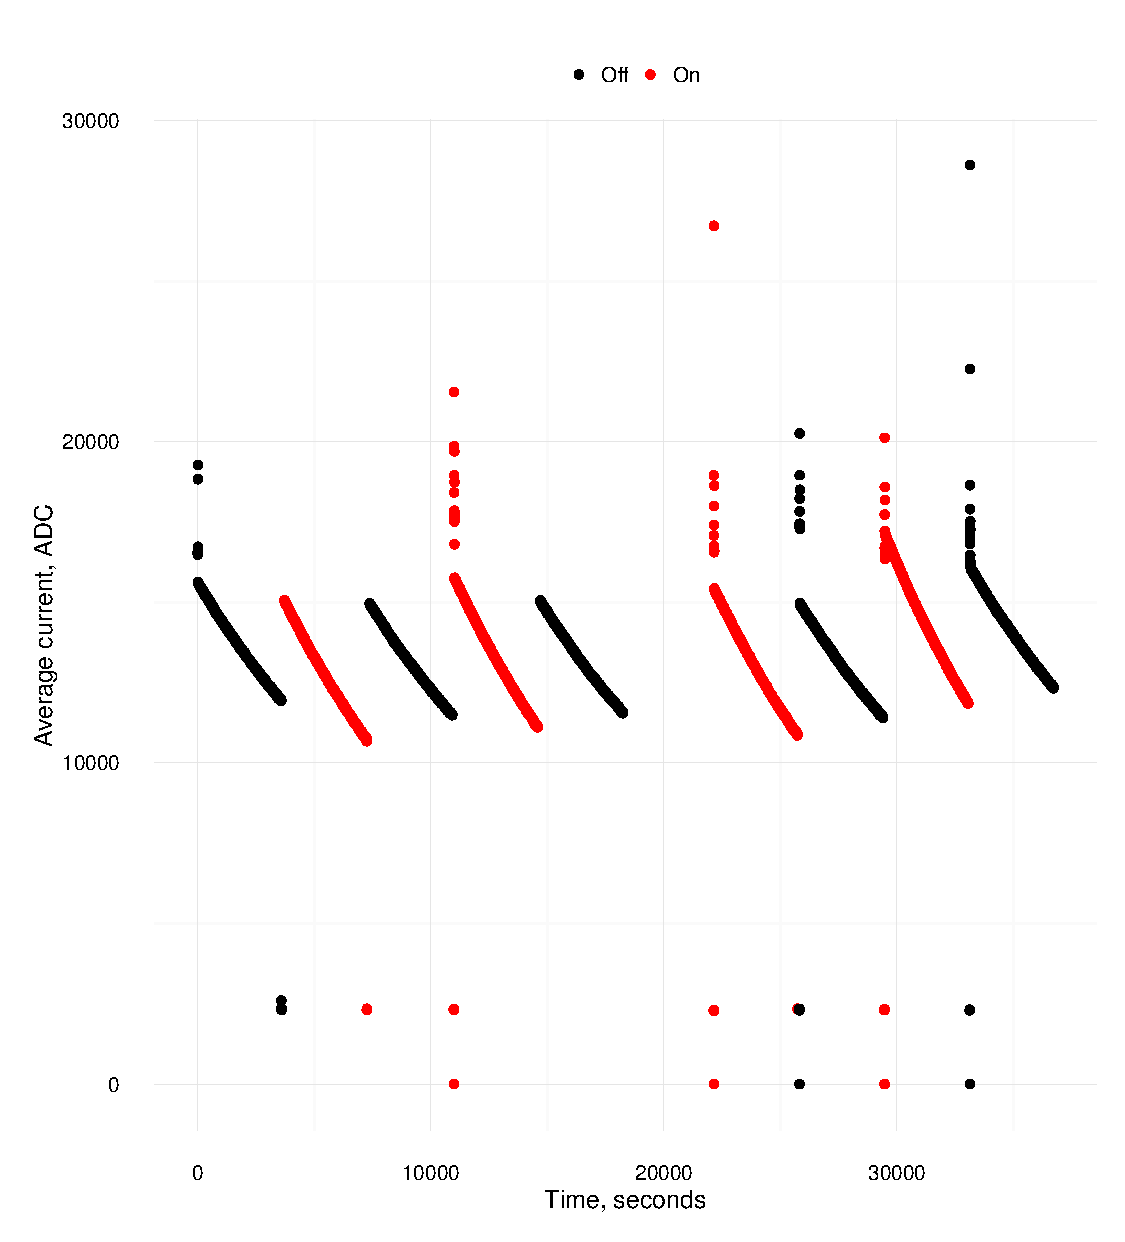
\includegraphics[scale=\scl]{../img/TheNineCycles}
\caption{The nine analyzed cycles.\label{fig:TheNine}}
\end{figure} 

The measurements were taken with a Beam Current Transformer (BCT). Based on inter-cycle data (baseline), it was concluded that the BCT offset systematically drifted toward zero by approximately 3.5 \ADCcode[s] per cycle during the cycles of interest.


\section{Estimation of slope}

To make correct slope estimates, we subtract offset $\Delta$ from the data. This is done  because
\begin{align*}
	\tilde{\slp} &= \frac{\td\ln \tilde{I}_t}{\td t} 
				  = \frac{1}{\tilde{I}_t}\frac{\td \tilde{I}_t}{\td t}, 
\shortintertext{where, if measured current}
	\tilde{I}_t  	&= I_t + \Delta_t = I_0\exp\bkt{\slp\cdot t} + \Delta_t, 
\shortintertext{then}
\tilde{\slp} 	&= \frac{1}{1 + \lambda_t}\bkt{\slp + \frac1{I_t}\frac{\td\Delta_t}{\td t}}, \\
	\lambda_t	&= {I_0}^{-1}\cdot \Delta_t\cdot\exp\bkt{-\slp\cdot t}.
\end{align*}

In the favorable case of a constant offset, it still must be removed in order to have a fixed estimate of slope. At this stage, estimation was done assuming offset was constant within a cycle, and only changed from cycle to cycle.

Since we did not have baseline data for two cycles, their offsets were estimated assuming a linear drift and fitting the cycles' baseline medians (FIG.~\ref{fig:OffsetModel}). Each cycle's data were subtracted its respective offset, and were fitted an ordinary least squares regression model of the form
\begin{equation}
	\ln\bkt{\tilde{I}_t} = \ln\bkt{I_0} + \slp\cdot t + \delta_t.
\end{equation}

\begin{figure}[h]
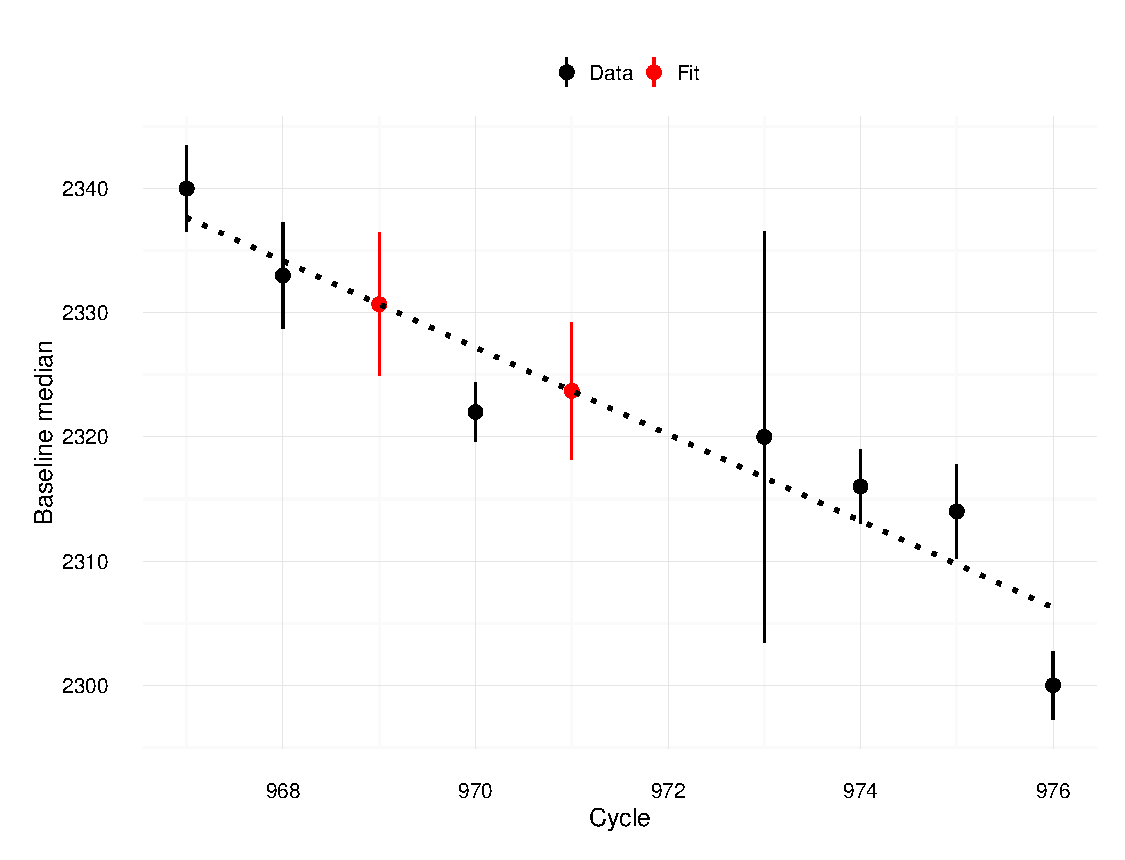
\includegraphics[scale=\scl]{../img/Offset_model_Common_GAM}
\caption{Offset model.\label{fig:OffsetModel}}
\end{figure}

The models' reduced chi-squares deviate from one in the fourth decimal place; however, one should note that the data do not pass linearity tests, and are likely to have structural slope changes as well (see TABLE~\ref{tbl:CycleChars}). Since the model residuals exhibit serial correlation (FIG.~\ref{fig:Run969}), the slope estimates' standard errors are estimated with robust estimators.

\begin{table}
\centering
\begin{threeparttable}
	\caption{Characteristics of a typical cycle.\label{tbl:CycleChars}}
	\begin{tabular}{llr}
	\hline\hline
	Charactetistic	& Test 					& P-value \\
	\hline
	Linearity 		& Harvey-Collier		& 0\% \\
	-				& Rainbow				& 0\% \\
	Constant slope	& Chow\tnote{a}		 	& 100\% \\
	-				& Moving estimates		& 1\% \\
	Homoskedasticity& Breusch-Pagan 		& 82\% \\
	Autocorrelation & Durbin-Watson			& 0\% \\
	\hline\hline
	\end{tabular}
	\begin{tablenotes}
	\item[a]{The Chow test was performed at every point in the fitting range. The average of F-statistics is used as the test statistic.}
	\end{tablenotes}
\end{threeparttable}
\end{table}


\begin{figure}
\centering
\begin{subfigure}{.5\textwidth}
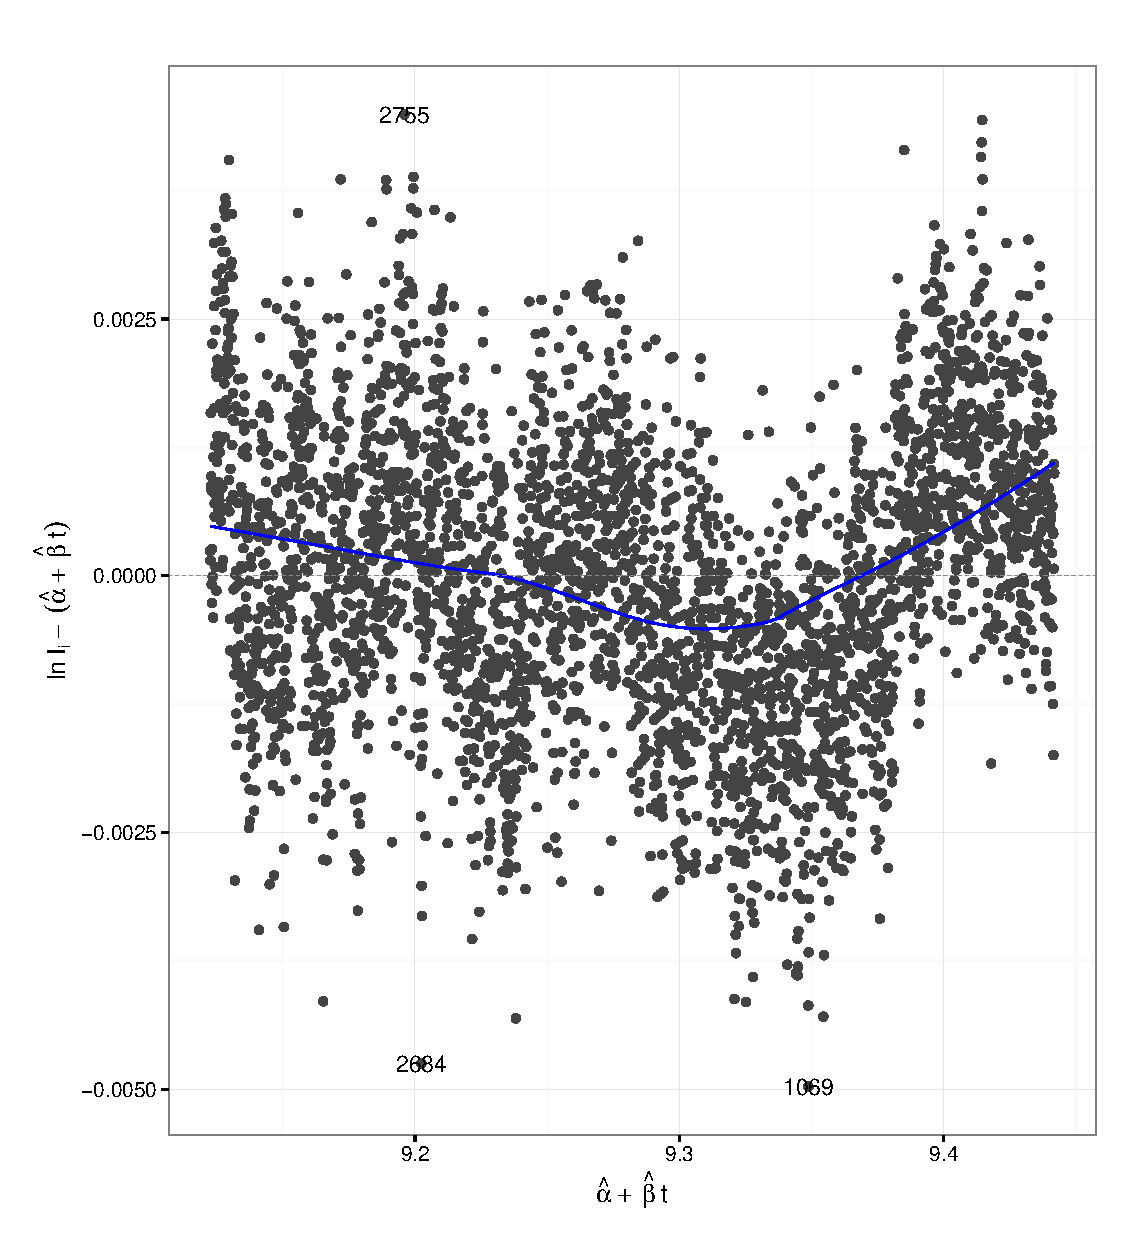
\includegraphics[scale=\scl]{../img/Run969_Res_VS_Fit}
\caption{Residuals vs fitted values.}
\end{subfigure}
\begin{subfigure}{.5\textwidth}
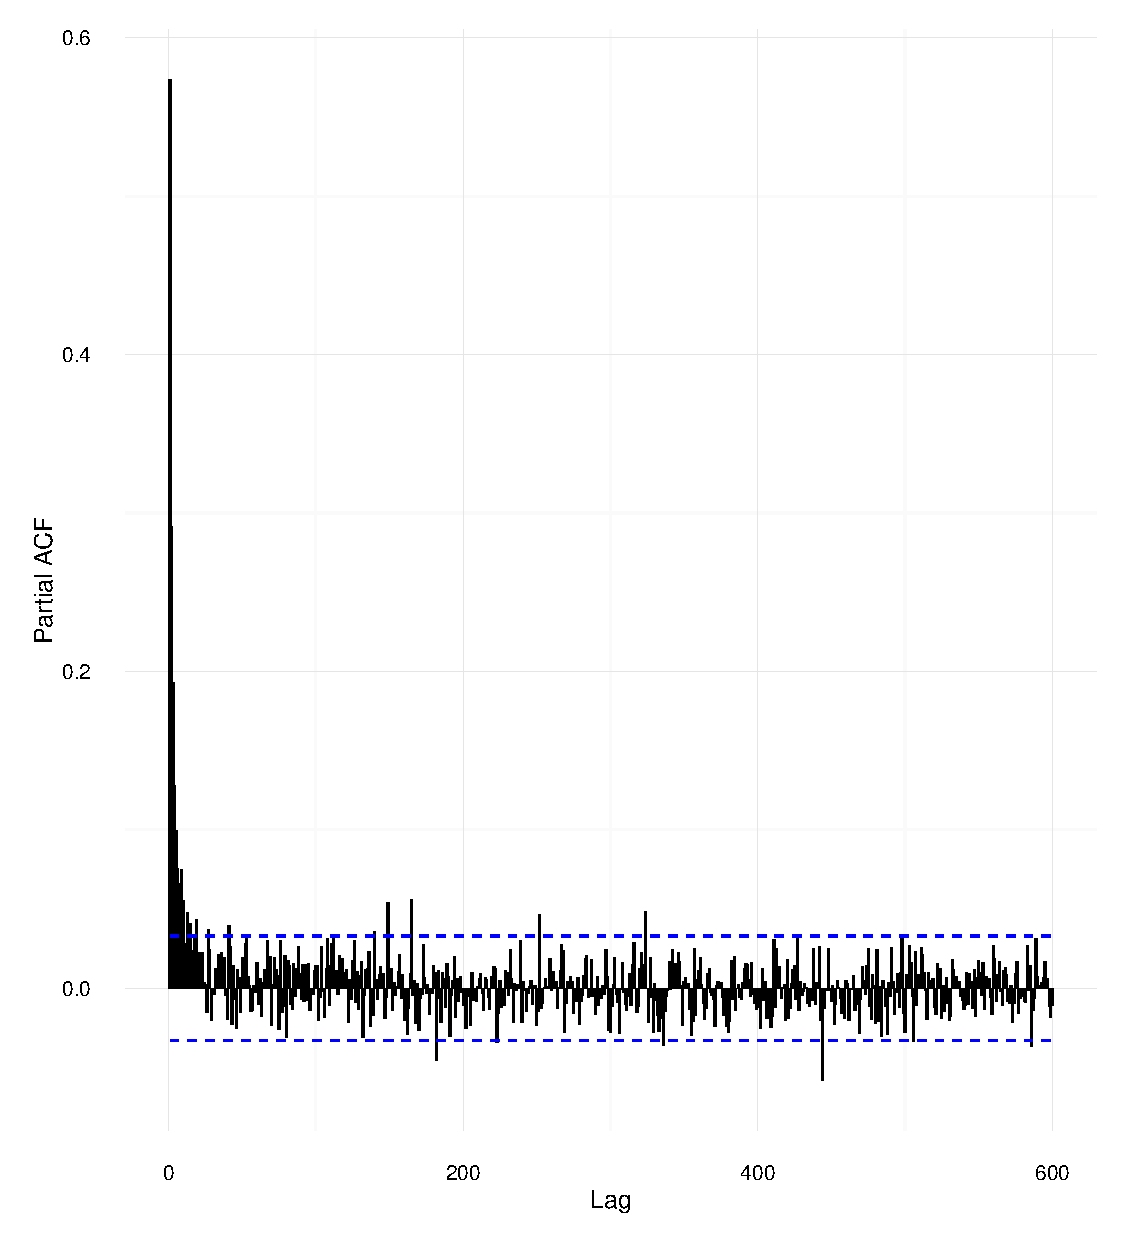
\includegraphics[scale=\scl]{../img/Run969_residual_PACF}
\caption{The partial Auto-Correlation Function of the residuals.}
\end{subfigure}
\caption{A typical cycle.\label{fig:Run969}}
\end{figure}

\section{Estimation of cross section}

In estimating cross section, only the estimates from adjacent cycles are used. This is done to minimize the effect of drifts of environmental variables such as target thickness, which is estimated to increase by $.5~ \sfrac{\%}{\mathrm{hour}}$. (The thickness by which the slope differences are divided, assumed constant, was provided by a Schottky measurement.)

This reduces the number of estimates from 20 to seven, of which three are deemed unsound according to Tukey's range test (with the range parameter corresponding to ten standard deviations). 

An estimate of a cross section estimate's standard error (SE) is made by adding the squared standard errors of the paired slopes, not taking account of the covariance term:
\begin{equation}
	\SE*{\CS*[0]} = \sqrt{\SE*{\slp*[off]}^2 + \SE*{\slp*[on]}^2}.
\end{equation}

This is done so because depending on whether an on-slope is paired with the preceding or succeding off-slope, the covariance term changes sign. Since there's no criterion favoring either of the two mappings, the covariance term was omitted.


\section{Results}

The summary statistics of cross section estimates, grouped by soundness and closeness of the slope estimates they are based on, are presented in TABLE~\ref{tbl:CS-all} and FIG.~\ref{fig:CS-all}. The slopes themselves are shown in FIG.~\ref{fig:Slopes}.

\begin{table}
\centering
\caption{Cross section estimates' statistics\label{tbl:CS-all}}
\begin{tabular}{llrcr}
\hline\hline
Soundness	& Closeness		& \#		& Mean (a.u.)		& SE (a.u.) \\
\hline
Sound		& Close			& 4			& 507				& 7  \\
Sound		& Far			& 8			& 549				& 14 \\
Unsound		& Close			& 3			& 560				& 39 \\
Unsound		& Far			& 5			& 518				& 20 \\
\end{tabular}
\end{table}

\begin{figure}
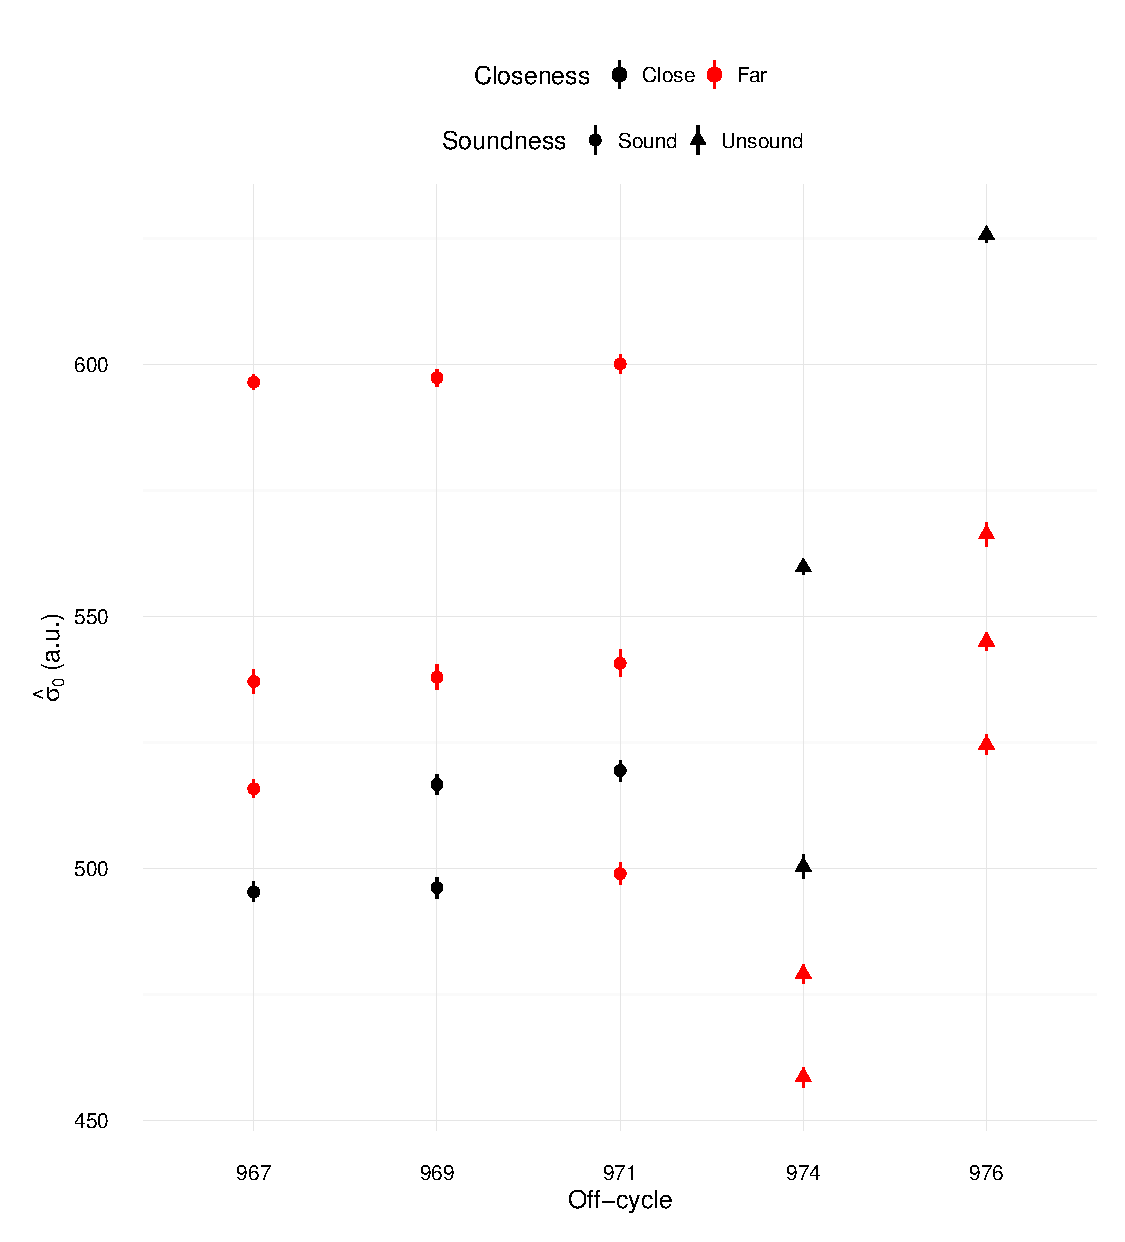
\includegraphics[scale=\scl]{../img/Cross-Section_all}
\caption{Cross section estimates.\label{fig:CS-all}}
\end{figure}%
\begin{figure}
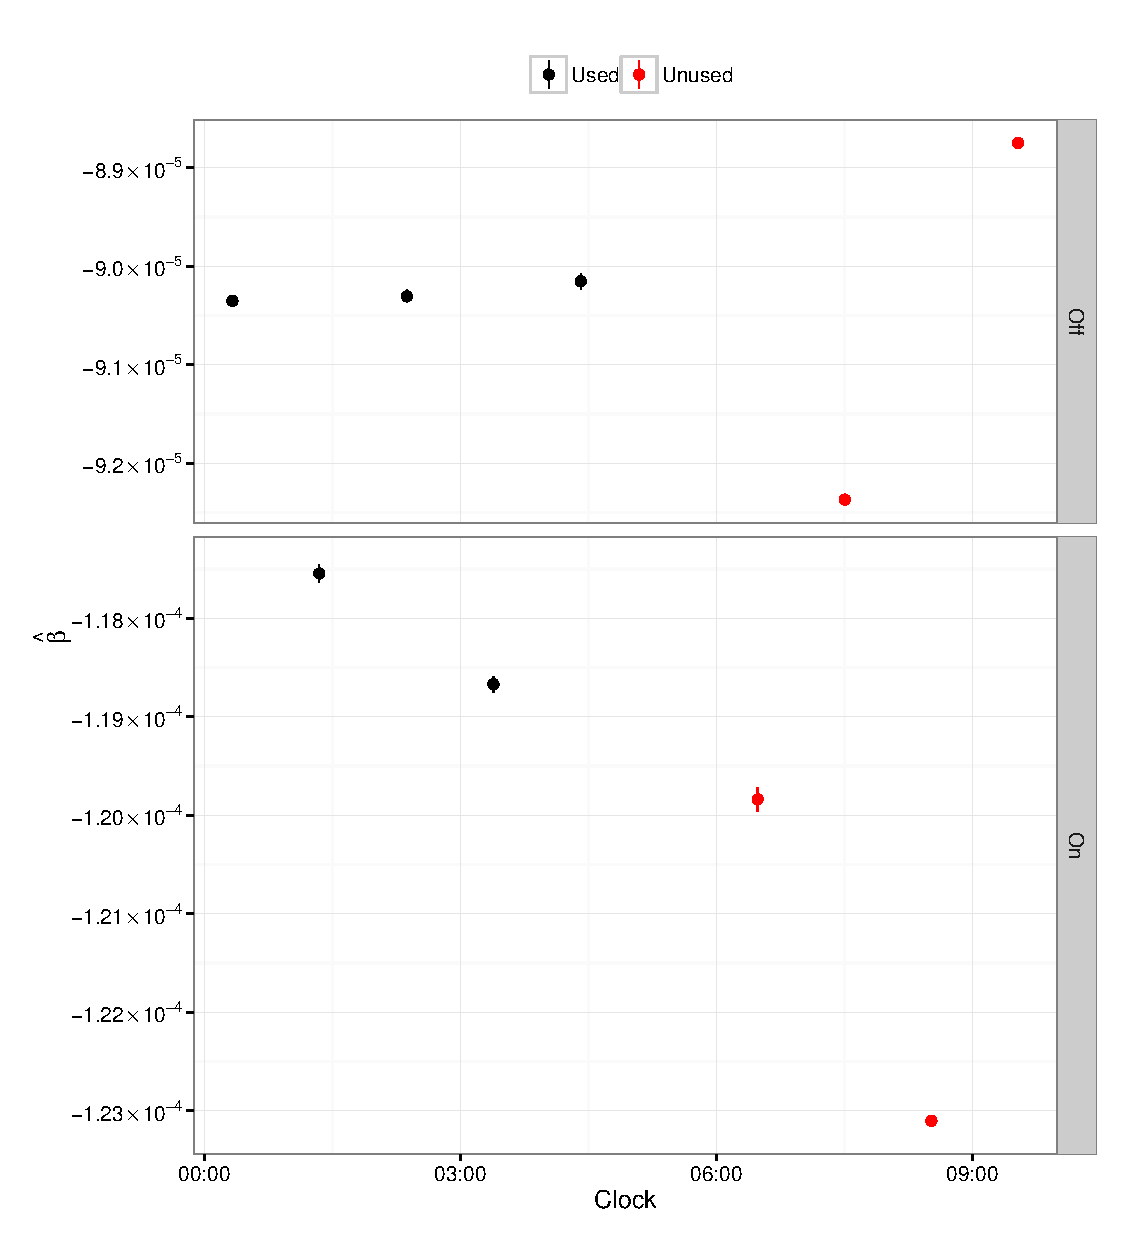
\includegraphics[scale=\scl]{../img/Slopes-2012_big}
\caption{Slope estimates.\label{fig:Slopes}}
\end{figure}


\end{document}
